% Document class `report-template` accepts either project-plan or final-report option in [].
\documentclass[project-plan]{report-template}

% Packages I use in my report.
\usepackage{graphicx}
\usepackage{amsmath}
\usepackage{blindtext}
\usepackage{subfig}
\usepackage{hyperref}
\usepackage{float}
\usepackage{caption}

\usepackage[square]{natbib}
\hypersetup{hidelinks}

% Directory where I saved my figures.
\graphicspath{{./figures/}}

% Metadata used for the title page - please modify.
\university{Imperial College London}
\department{Department of Earth Science and Engineering}
\course{MSc in Applied Computational Science and Engineering}
\title{Deep Learning Algorithms Applied to Surface Mapping of Mars}
\author{Niranjana Sundararajan}
\email{niranjana.sundararajan21@imperial.ac.uk}
\githubusername{acse-ns1321}
\supervisors{Dr Cédric M. John\\
Dr Philippa J. Mason}
\repository{https://github.com/ese-msc-2021/irp-acse-ns1321}

\begin{document}

\maketitlepage  % generate title page

% Abstract
\section*{Abstract}

An accurate understanding of Martian Terrain and its features is crucial not only to further  scientific research in the fields of planetary science but also essential to engineers responsible for planning rover landings and building models for landing site traversability analysis. While current tools and research provide for supervised classification of landforms and features based on known/suspected terrain classifiactions,these often fail to acknowdlege the possiblilty that Martian terrains may exhibit features that are significantly different from our present understanding of terrains. 
Using the Mars Reconissance Orbiter's HIRISE images that have a resolution of 25cm/pixel, this project focuses on first create a publically available API package to download the images and extract hidden patterns and features in the images using a deep learning based encoding algorithm such as a convolutional neural network or an autoencoder.Consequently the images are categorised using a clustering algorithms such as K Means and DBSCAN based on similarity of their derived features.
Therefore this model will provide researchers and engineers alternative ways to study unique features in Martian Terrains. 


% Introduction section
\section{Introduction}

The Martian Terrain, much like earth, possesses a multitude of landscape features. The United States Geological Survey has divided the Martian land into thirty quadrangles, each defined by a specific latitude and longitude. NASA/JPL/MSSS have created a map shown below:
\begin{figure}[h]
    \begin{center}
        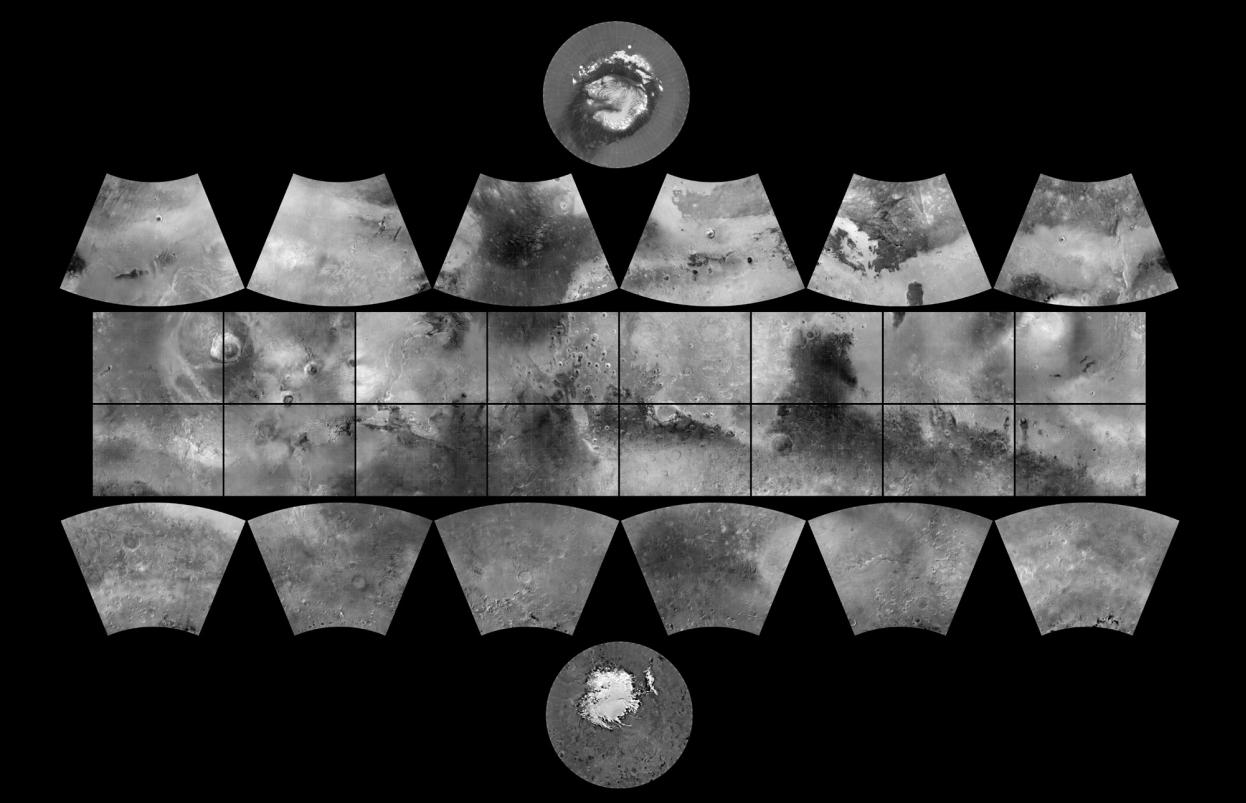
\includegraphics[width=1\textwidth]{quadrangles-NASA-JPL-MSSS.jpg}
    \end{center}
    \caption{\label{fig:Martian Quadrangles} The MGS MOC Wide Angle Map of Mars. Source : NASA/JPL/MSSS }
\end{figure}

 Some of the characteristic features of the terrain include volcanos, canyons, impact craters and dry lake beds. A brief study of the main features studied in preparation for this project based on availabe information are summarized in the tables that follow: \\

 \begin{figure}[htp]
    \begin{center}
        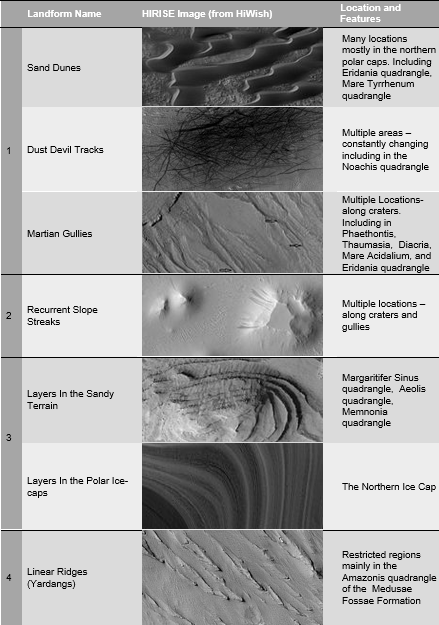
\includegraphics[width=1\textwidth]{table-1-part-1.png}
    \end{center}
\end{figure}

\begin{figure}[htp]
    \begin{center}
        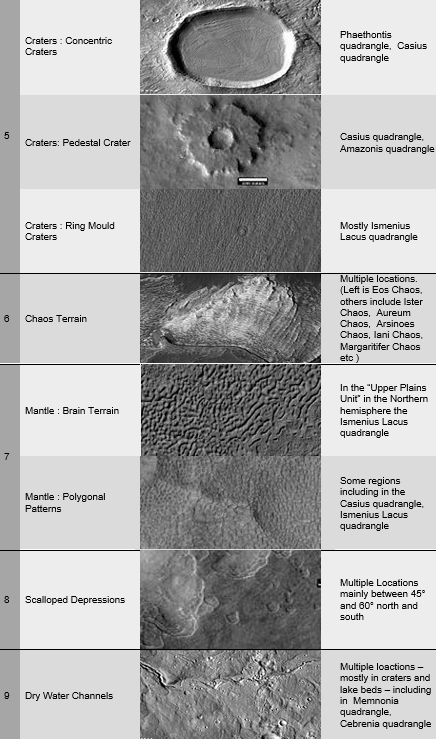
\includegraphics[width=1\textwidth]{table-1-part-2.png}
    \end{center}
\end{figure}

\begin{figure}[htp]
    \begin{center}
        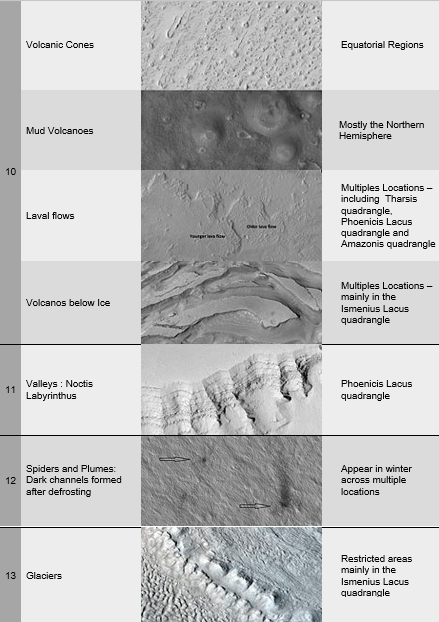
\includegraphics[width=1\textwidth]{table-1-part-3.png}
    \end{center}
\end{figure}

Presently, there are mainly two types of research objectives that are considered while building deep learning models involving martian terrains. \\
In the first kind, researchers have used automated image analysis and deep learning techniques for the detection of specific terrain features such as dunes fields \citep{5692810}, craters \citep{Lee_2019,palafox2015automated}, volcanic cones \citep{palafox2015automated} and aeolian ridges \citep{palafox2017automated}. 
In the second, researches have used deep learning algorithms to build supervised algorithms that classify availabe images into defined classes. The Soil Property and Object Classification \citep{Rothrock2016SPOCDL} software  successfully classifies full resolution HIRISE images into 17 terrain classes using a specialized Fully Convolutional Neural Network.

A major shortcoming in these generalized classifiers using convolutional neural networks is that these models, that are supervised by nature, require images to be manually labelled before training. Therefore considering the total data volume and the abundance of new images, even the recent, more accurate classifiers such as those deployed within the Planetry Data System's Imaging Atlas \citep{Wagstaff2018DeepMC}  will likley fail to account for newly captured features. \\



% Another section
\section{Problem Description and Objectives}
This project aims to build a classification model that takes in as input a set of preprocessed HIRISE images, extract and encode the features and image information and finally using clustering methods separate them into an appropriate number of unlabelled classes. The schematic of the proposed model stages can be seen below :\\

\begin{figure}[htp]
    \begin{center}
        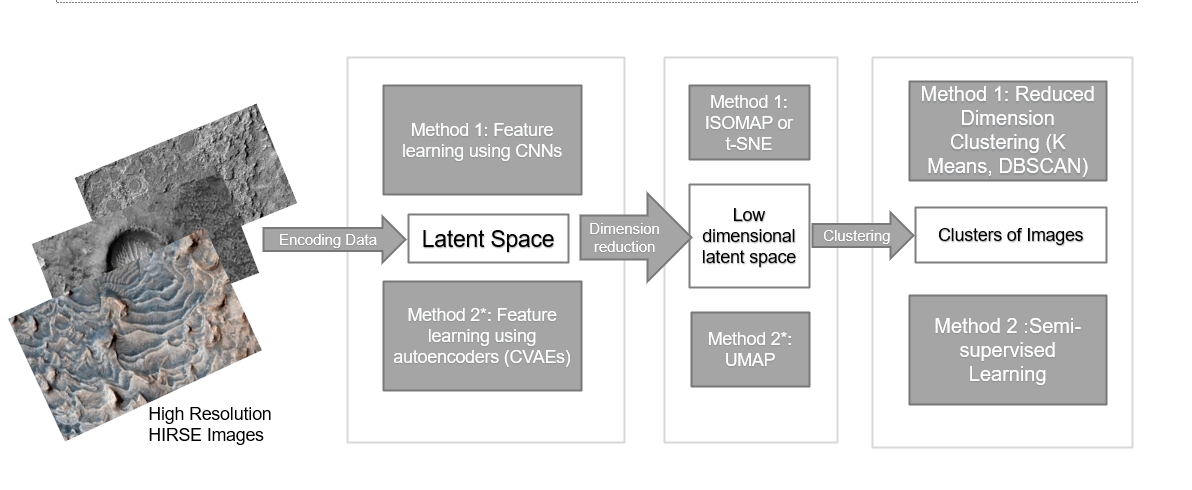
\includegraphics[width=1.1\textwidth]{model-schematic.png}
        \caption{\label{fig:Model Schematic} The Proposed Model Development Schematic }
    \end{center}
\end{figure}


The \textbf{first objective } in building this model is the injestion of the HIRISE images and the associated metadata. The proposed solution is the building of a python package designed based on Object Oriented Programming principles that allows for easy queying and downloads. The tool allows the user to webscrape the necessary file hierarchies from the websites as well as create an updatable database that holds all the currently available information. Building this tool has been the focus of the project so far. \\

The \textbf{second stage} and an important objective of this project is to find a deep learning algorithm that allows for appropriate encoding of the image data, such that the features are preserved and feature selection can be executed with accpetable results while decoding. Considering that the images in the HIRISE database range from 1Gb to 87Gbs, it is essential that this encoding not only captures features correctly but also allows for dimension reduction after latent space generation. Of the encoding algorithms available(including convolutional neural networks), autoencoders, specifically the convolutional variational autoencoder(CVAE), due to their stability and ability to retain spatial information show great promise for this purpose. While using a regular autoencoder has shown to produce good results when used for pre-training on Martian Terrains\citep{Rothrock2016SPOCDL} as well as its proven suitability for dimension reduction purposes\citep{WANG2016232}, it will be interesting to observe how much better a CVAE performs on these images. \\

Once the high dimensional latent space is generated, the \textbf{third stage} is to use projection based dimension reduction techniques such as Isomaps, t-distributed stochastic neighbour embedding(t-SNE) or the most approprite a Uniform Manifold Approximation and Projection(UMAP) that has demonstrated structure preservation on Mars images\citep{Allaoui2020ConsiderablyIC}. UPMAPs, in contrast to t-SNEs, compresses the high dimensional latent space  instead of converting it point by point. This makes the process more computationally efficient.

The \textbf{fourth stage} in building the model is the selection of a clustering algorithm that will classsifiy the reduced and encoded latent space of images. The two possible operations include a reduced dimension clustering method such as K Means or DBSCAN that has previously shown good results for high resolution remote sensing images \citep{ZHANG201675}, or a semi-supervised learning algorithm that uses transfer learning, which is a pretrained network to group images into clusters.

In summary, the potential challenges that are likley to be encountered  besides the preprocessing of the data are the selection of encoding methods, selection of a appropriate clustering algorithms and choosing the most appropriate performance metrics. More importantly, a special consideration is to be given for ease of use of the package and the reproducibility and scalabilty of the code, which will not only allow future researchers to use the existing tool for future classifications but also allow researchers to expand the tool's use to support their own research. 



\section{Progress to Date and Future Plan}
 HIRISE is a growing databse of images - presently populated with over 73,000 images and over 25 parameters that define each image. To be able to consume this data it was imperative to build a tool that allows for easy access to required images and their associated metadata. The Planetary Data System(PDS), maintained by NASA, while allowing the user to browse the catalogues of available information requires the user to manually navigate to specific folders and download single images. This is tedious and time-consuming. \\
 This project implements a package that allows for these functions. It currently includes 32 querying functions, with additonal functions that allow for downloading the current database, updating the current database with new information from the PDS and downloading filtered/specified images directly. It also includes a package for preprocessing the image data that has functions such as tiling, resizing to zoom in/out on images (staring from 25cm/pixel to 250+ cm/pixel), loading the pytorch dataset, converting to grayscale etc. \\

 The aim is to build the software using agile methodologies and lean software development. Based on the agile manifesto the following are a few practices that were observed and implemented : \\
 \begin{itemize}
    \item \textbf{Continuous Delivery}: In order to obtain frequent feedback and facilitate continuous improvement multiple verions of the software were released during the development process. Presently there are 28 different verisons availabe on the pypi test wesbite with a progressive improvement and bug fixes noted with each version,
    \item \textbf{Problem Breakdown}: The software was developed first by planning the overarching architectture of features and functions required, then  individual classes, their associated functions and utility modules were planned and executed in stages. The code undergoes refactoring and optimisations when the logic is complete
    \item \textbf{Measuring Progress} : Planning and progress is meaured through GIT's project board. This a Kanban Style board developed by git to aid lean software development by allowing for task breakdown, distribution, progress evaluation, commenting  and feedback.
 \end{itemize}

 The next steps include expanding on the preprocessing package with functions such as cropping preprossed images, splitting the data into train and test sets taking into account spatial correlation, encoding using CVAEs, dimensionality reduction using UMAPS etc. These functions can then access the hirise image objects which will serve as inputs to these functions.\\
 The step following the implementation of the preprocessing package will be another class associated with training that will perform the clusering based on the algorithm chosen. Finally based on the specifics of the implemented algorithm there will be a final class that calculates accuracy metrics and provies the user with information on how well the algorithm has performed. \\

 The gantt charts below demonstrate the planned implementation of the different stages of the project for the coming months: \\

\begin{figure}[htp]
    \begin{center}
        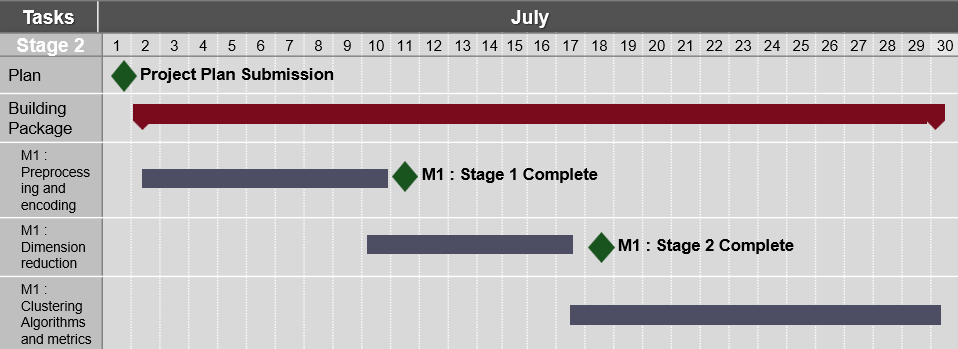
\includegraphics[width=0.7\textwidth]{gantt-july.png}
        \caption{}{Proposed Gantt Chart for July} 
    \end{center}
\end{figure}

\begin{figure}[htp]
    \begin{center}
        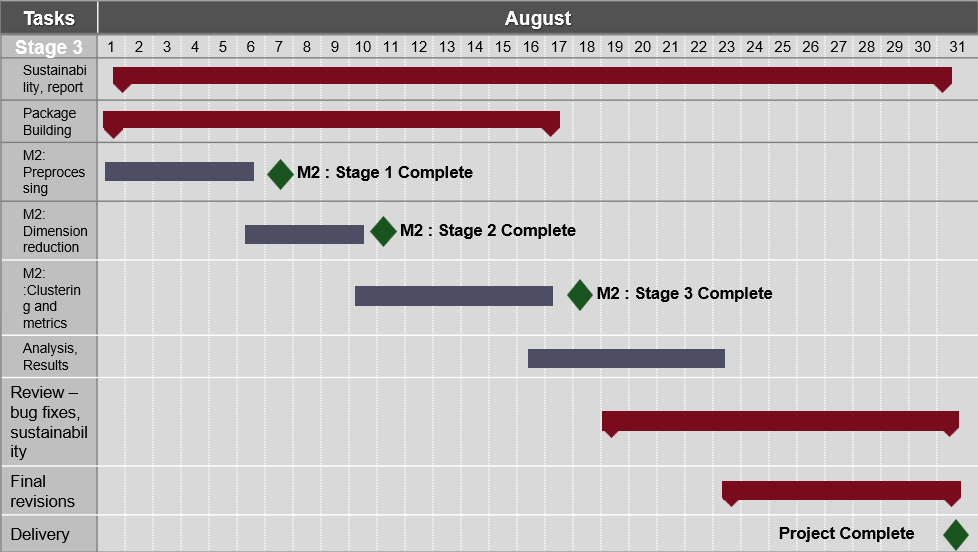
\includegraphics[width=0.7\textwidth]{gantt-august.png}
        \caption{}{Proposed Gantt Chart for August} 
    \end{center}
\end{figure}


% References
\nocite{*}
\bibliographystyle{cell}
\bibliography{references}  % BibTeX references are saved in references.bib

\end{document}          
